\section{Integrali po \texorpdfstring{$\omega$}{ω}-kompleksih}
\subsection{Definicija}
\begin{definicija}
  Neskončno zaporedje kompleksnih števil, označeno z $\omega = (\omega_1, \omega_2, \ldots)$,
  se imenuje \emph{$\omega$-kompleks}.\footnote{To ime je izmišljeno.}

  Črni blok zgoraj je tam namenoma. Označuje, da \LaTeX{} ni znal vrstice prelomiti pravilno
  in vas na to opozarja. Preoblikujte stavek ali mu pomagajte deliti problematično besedo z
  ukazom \verb|\hyphenation{an-ti-ko-mu-ta-ti-ven}| v preambuli.
\end{definicija}
\begin{trditev}[Znano ime ali avtor]
  \label{trd:obstoj-omega}
  Obstaja vsaj en $\omega$-kompleks.
\end{trditev}
\begin{proof}
  Naštejmo nekaj primerov:
  \begin{align}
    \omega &= (0, 0, 0, \dots), \label{eq:zero-kompleks} \\
    \omega &= (1, i, -1, -i, 1, \ldots),  \\
    \omega &= (0, 1, 2, 3, \ldots). \qedhere  % postavi QED na zadnjo vrstico enačbe
  \end{align}
\end{proof}
\section{Tehnični napotki za pisanje}
\subsection{Sklicevanje in citiranje}
Za sklice uporabljamo \texttt{\\ref}, za sklice na enačbe \texttt{\\eqref}, za citate \texttt{\\cite}. Pri
sklicevanju in citiranju sklicano številko povežemo s prejšnjo besedo z nedeljivim presledkom
$\sim$, kot npr.\ \verb|iz trditve~\ref{trd:obstoj-omega} vidimo|.

\begin{primer}
  Zaporedje~\eqref{eq:zero-kompleks} iz dokaza trditve~\ref{trd:obstoj-omega} na
  strani~\pageref{trd:obstoj-omega} lahko najdemo tudi v Spletni enciklopediji zaporedij~\cite{oeis}.
  Citiramo lahko tudi bolj natančno~\cite[trditev 2.1, str.\ 23]{lebedev2009introduction}.
\end{primer}

\subsection{Okrajšave}
Pri uporabi okrajšav \LaTeX{} za piko vstavi predolg presledek, kot npr. tukaj. Zato se za vsako
piko, ki ni konec stavka doda presledek običajne širine z ukazom \verb*|\ |, kot npr.\ tukaj.
Primerjaj z okrajšavo zgoraj za razliko.

\subsection{Vstavljanje slik}
Sliko vstavimo v plavajočem okolju \texttt{figure}. Plavajoča okolja \emph{plavajo} po tekstu, in
jih lahko postavimo na vrh strani z opcijskim parametrom `\texttt{t}', na lokacijo, kjer je v kodi s
`\texttt{h}', in če to ne deluje, potem pa lahko rečete \LaTeX u, da ga \emph{res} želite tukaj,
kjer ste napisali, s `\texttt{h!}'. Lepo je da so vstavljene slike vektorske (recimo \texttt{.pdf}
ali \texttt{.eps} ali \texttt{.svg}) ali pa \texttt{.png} visoke resolucije (več kot
\unit[300]{dpi}).  Pod vsako sliko je napis in na vsako sliko se skličemo v besedilu. Primer
vektorske slike je na sliki~\ref{fig:sample}. Vektorsko sliko prepoznate tako, da močno
zoomate v sliko, in še vedno ostane gladka. Več informacij je na voljo na
\url{https://en.wikibooks.org/wiki/LaTeX/Floats,_Figures_and_Captions}. Če so slike bitne, kot na
primer slika~\ref{fig:image}, poskrbite, da so v dovolj visoki resoluciji.

\begin{figure}[h]
  \centering
  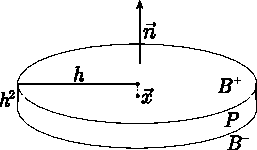
\includegraphics[width=0.6\textwidth]{images/sample.pdf}
  % \caption[caption za v kazalo]{Dolg caption pod sliko}
  \caption[Primer vektorske slike.]{Primer vektorske slike z oznakami v enaki pisavi, kot jo
     uporablja \LaTeX{}.  Narejena je s programom Inkscape, \LaTeX{} oznake so importane v
     Inkscape kot PDF, narejen s pomožno \texttt{.tex} datoteko.}
  \label{fig:sample}
\end{figure}

\begin{figure}[h]
  \centering
  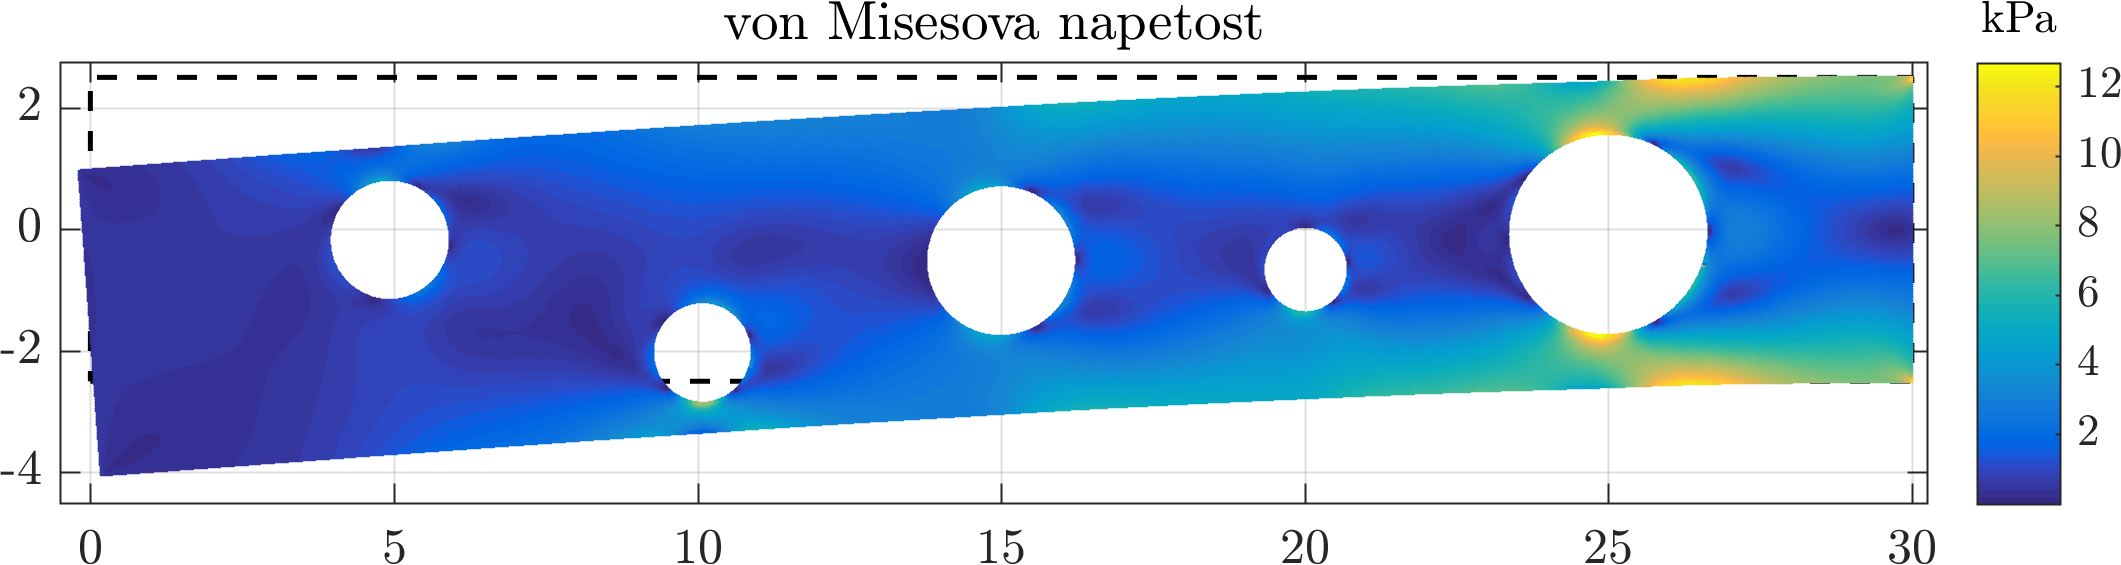
\includegraphics[width=0.8\textwidth]{images/image.png}
  \caption[Primer bitne slike.]{Primer bitne slike, izvožene iz Matlaba. Poskrbite, da so slike v
  dovolj visoki resoluciji in da ne vsebujejo prosojnih elementov (to zahteva PDF/A-1b format).}
  \label{fig:image}
\end{figure}

\subsection{Kako narediti stvarno kazalo}
Dodate ukaze \verb|\index{polje}| na besede, kjer je pojavijo, kot tukaj\index{tukaj}.
Več o stvarnih kazalih je na voljo na \url{https://en.wikibooks.org/wiki/LaTeX/Indexing}.

\subsection{Navajanje literature}
Članke citiramo z uporabo \verb|\cite{label}|, \verb|\cite[text]{label}| ali pa več naenkrat z
\verb|\cite{label1, label2}|.
Tudi tukaj predhodno besedo in citat povežemo z nedeljivim presledkom
$\sim$. Na primer~\cite{chen2006meshless,liu2001point}, ali pa \cite{kibriya2007empirical}, ali pa
\cite[str.\ 12]{trobec2015parallel}, \cite[enačba (2.3)]{pereira2016convergence}.
Vnosi iz \verb|.bib| datoteke, ki niso citirani, se ne prikažejo v seznamu literature, zato jih
tukaj citiram.~\cite{vene2000categorical}, \cite{gregoric2017stopniceni}, \cite{slak2015induktivni},
\cite{nsphere}, \cite{kearsley1975linearly}, \cite{STtemplate}, \cite{NunbergerTand}, \cite{vanoosten2008realizability}.
